\chapter{Contexte général}
\section*{Introduction}



Dans ce premier chapitre, nous allons poser les bases de notre travail en explorant son contexte général. Nous débuterons par une présentation de l’organisme d’accueil, la société SIGA, en mettant en lumière son domaine d’expertise et son rôle. Ensuite, nous introduirons le projet en détail, avant d’examiner l’existant afin d’identifier ses limites et les opportunités d’amélioration que notre solution vise à concrétiser. Enfin, nous exposerons la méthodologie suivie pour concevoir ce projet ainsi que les grandes lignes de la solution proposée.



  
% Une section

% Exemple d'une section qui porte une référence à une bibliographie
% NB: il faut bien suivre le syntaxe pour ne pas tomber dans le cas où il y a une référence dans la table des matières.
\section[Organisme d'accueil]{Organisme d'accueil}

\subsection{SIGA}

Créée en 1996, SIGA (Système Informatique et Gestion Automatisée) s’est imposée comme un acteur majeur dans le domaine du développement de logiciels et des solutions informatiques en Tunisie. Basée à Tunis, l’entreprise regroupe une équipe de plus de vingt ingénieurs et six consultants seniors, cumulant entre 5 et 25 ans d’expérience dans la conception et l’intégration de systèmes d’information. Depuis sa fondation, SIGA se distingue par son expertise multidisciplinaire, offrant des services qui couvrent l’ensemble du cycle de vie d’un produit informatique : de l’analyse des besoins à la mise en œuvre, en passant par le développement, la formation et la maintenance.
\begin{figure}[H]
\centering
\includegraphics[scale=0.5]{images/siga.png}
\caption{Logo de SIGA}
\label{fig:Siga_logo}
\end{figure}
    \newpage
\subsection{Secteur d'activité}
SIGA déploie son expertise dans divers secteurs, proposant des solutions technologiques adaptées aux besoins spécifiques de ses clients. Ses principaux domaines d’intervention incluent :
\begin{itemize}
    \item \textbf{Banque et assurance : }développement de systèmes pour optimiser la gestion des processus financiers et administratifs.
    \item \textbf{Industrie : }conception de logiciels pour améliorer la gestion de la production et des ressources.
    \item \textbf{Transports : }mise en place de solutions facilitant la logistique et la coordination opérationnelle.
    \item \textbf{Télécommunications : }création de systèmes pour rationaliser les interactions et la gestion des données.
    \item \textbf{Autres secteurs :}accompagnement à la digitalisation des opérations pour des entreprises variées, avec une présence étendue en Tunisie et dans plusieurs pays africains (Mali, Côte d’Ivoire, Tchad, Mauritanie).
\end{itemize}

\section{Présentation du Projet}
Le projet que j’ai réalisé s’inscrit dans le cadre de mon projet de fin d’études en dernière année à l’École Supérieure Privée d’Ingénierie et de Technologie (ESPRIT). J’ai effectué mon stage au sein de SIGA, une entreprise reconnue pour son expertise dans le développement de logiciels et de solutions informatiques innovantes en Tunisie.

Dans cette section, nous présentons notre projet en détaillant, dans un premier temps, un aperçu du « Portail de Gestion des Approbations avec Workflows Dynamiques et Déploiement Automatisé » et ses spécificités. Dans un second temps, nous aborderons la problématique, l’étude de l’existant, notre contribution ainsi que la méthodologie adoptée pour mener à bien cette mission.
\subsection{Présentation du Portail de Gestion des Approbations}
Le projet « Portail de Gestion des Approbations avec Workflows Dynamiques et Déploiement Automatisé » est une solution conçue pour centraliser et optimiser la gestion des processus d’approbation au sein des organisations. Son objectif principal est de simplifier la soumission, le suivi et la validation des demandes – telles que les congés ou les autorisations – en offrant une interface intuitive et des mécanismes automatisés. Ce portail se distingue par sa capacité à adapter dynamiquement les workflows en fonction des besoins spécifiques de chaque demande, garantissant ainsi une flexibilité et une personnalisation optimales.\\
\\
    \newpage
Le portail prend en charge divers types de demandes et génère des outputs variés, notamment des notifications par email ou push notification, des statuts en temps réel, et des rapports analytiques sous forme de tableaux de bord. À terme, il vise à gérer un volume significatif de requêtes quotidiennes tout en assurant une traçabilité complète des actions effectuées. Développé avec Angular pour le frontend, Spring Boot pour le backend, et Camunda pour l’orchestration des workflows, le système repose sur une architecture moderne déployée via Docker et orchestrée par Kubernetes. Il est hébergé sur plusieurs environnements distincts : développement (DEV), tests (TEST) et production (PROD), avec une infrastructure évolutive adaptée à chaque contexte.\\
\\
Chez SIGA, ce projet joue un rôle clé dans la digitalisation des processus internes, et toute interruption pourrait affecter la fluidité des opérations, rendant sa disponibilité une priorité essentielle.

\subsection{Spécificités du Portail de Gestion des Approbations}
Le portail est un outil de gestion des processus qui permet aux utilisateurs de soumettre et de suivre des demandes via différents canaux et fonctionnalités, notamment : \begin{itemize}
    \item \textbf{Workflows dynamiques: }des processus personnalisables définis avec Camunda.
    \item \textbf{Suivi en temps réel: }un statut actualisé et un historique des actions.
    \item \textbf{Reporting: }des tableaux de bord pour analyser les processus.
    \item \textbf{Notifications: }des alertes automatiques par email ou temps réel.
\end{itemize}
\subsection{ Problématique } 
Dans de nombreuses organisations, les processus d’approbation sont encore réalisés de manière manuelle. Cela engendre plusieurs problématiques :
\begin{itemize}
  \item \textbf{Lenteur des traitements: }Les délais sont souvent rallongés à cause des allers-retours entre les différents acteurs.
  \item \textbf{Manque de traçabilité :} Il est difficile de connaître l’état d’avancement d’une demande ou de retracer les actions passées.
  \item \textbf{Risque d’erreurs humaines : }En raison du manque d’automatisation, certaines étapes peuvent être oubliées ou mal exécutées.
\end{itemize}

\subsection{ Situation actuelle et Critiques } 
Actuellement, pour obtenir une approbation (congé, autorisation...), le processus suit généralement les étapes suivantes :
\begin{enumerate}
    \item Remplissage manuel d’un formulaire papier ou d’un document bureautique (Word, Excel).
    \item Transmission physique ou par email au supérieur hiérarchique.
    \item Approbation manuelle, parfois verbale, sans traçabilité.
    \item Notification au demandeur uniquement si ce dernier relance.
\end{enumerate}
\subsubsection*{Inconvénients:}
\begin{itemize}
    \item \textbf{Non-centralisation} : Les demandes sont éparpillées (emails, papiers, discussions).
    \item \textbf{Perte de temps} : Les relances sont fréquentes.
    \item \textbf{Absence de supervision globale} : Aucune visibilité d’ensemble pour l’administration.
    \item \textbf{Aucune possibilité d’analyse} : Pas de données statistiques sur les demandes, les délais, les refus, etc.
\end{itemize}

\section{Solution proposée}

Afin de répondre aux limites identifiées dans le processus actuel, il est proposé de mettre en place un \textbf{Portail Web de Gestion des Approbations} moderne, centralisé et automatisé. Ce portail repose sur une architecture modulaire et des technologies éprouvées pour assurer une solution performante, évolutive et facilement maintenable.

\subsection*{Automatisation des workflows avec Camunda BPM}

Le cœur de la solution repose sur l'intégration de \textbf{Camunda BPM}, un moteur de workflow open-source basé sur le standard BPMN (Business Process Model and Notation). Chaque type de demande (congé, achat, autorisation, etc.) est modélisé sous forme de processus graphique. Ces workflows définissent les différentes étapes à suivre, les rôles impliqués et les règles de validation.

L’utilisation de Camunda permet :
\begin{itemize}
    \item La \textbf{définition claire et visuelle} des processus métiers.
    \item L’\textbf{exécution automatique} des étapes selon les règles définies.
    \item La \textbf{flexibilité} de modifier les processus sans redéployer l’application.
    \item L’\textbf{assignation dynamique} des tâches aux utilisateurs concernés.
\end{itemize}

\subsection*{Digitalisation de la soumission des demandes}

L’interface utilisateur, développée avec \textbf{Angular}, permet aux utilisateurs de soumettre leurs demandes via des formulaires en ligne ergonomiques et adaptés au type de demande. Chaque formulaire est connecté à une instance de processus Camunda qui orchestre automatiquement les étapes suivantes. Cette digitalisation permet de :
\begin{itemize}
    \item Réduire les erreurs de saisie grâce à des contrôles intégrés.
    \item Gagner du temps en supprimant les supports papier.
    \item Standardiser la soumission et le traitement des demandes.
\end{itemize}
\newpage
\subsection*{Suivi en temps réel et notifications automatiques}

Chaque utilisateur peut suivre en temps réel le statut de ses demandes (approuvée, rejetée ou en cours de traitement). Le portail intègre un système de \textbf{notifications en temps réel} directement dans l’interface de l’application, basé sur des technologies de type WebSocket:

\begin{itemize}
    \item Alerte à l'approbateur lorsqu’une tâche lui est assignée.
    \item Notification au demandeur une fois la décision prise.
    \item Rappels pour les tâches non traitées dans un délai défini.
\end{itemize}

Ce mécanisme renforce la réactivité des acteurs et limite les retards.

\subsection*{Infrastructure moderne, scalable et résiliente}

L’ensemble de l’application est conteneurisé à l’aide de \textbf{Docker} afin de garantir une portabilité maximale et un déploiement simplifié. Le déploiement se fait sur un cluster \textbf{Kubernetes} pour bénéficier :
\begin{itemize}
    \item D’une haute disponibilité des services.
    \item D’un équilibrage de charge automatique.
    \item D’une scalabilité horizontale en fonction de la charge.
\end{itemize}

\subsection*{Pipeline DevOps pour l’intégration et le déploiement continus}

Un pipeline CI/CD est mis en place avec \textbf{ArgoCD} pour automatiser :
\begin{itemize}
    \item La compilation et les tests des composants backend et frontend.
    \item La construction des images Docker.
    \item Le déploiement automatique sur l’environnement de production.
\end{itemize}

Cela permet de garantir la rapidité, la fiabilité et la répétabilité du processus de livraison.

\subsection*{Analyse des performances et tableaux de bord}

Des tableaux de bord sont mis à disposition des administrateurs pour visualiser :
\begin{itemize}
    \item Le nombre de demandes traitées par type ou par service.
    \item Les délais moyens de traitement.
    \item Les goulets d’étranglement dans les workflows.
\end{itemize}

Ces indicateurs permettent d’optimiser les processus métier et de prendre des décisions basées sur des données concrètes.


\newpage
\section{Méthodologie de gestion de projet}
\normalsize{

Afin d'assurer le bon déroulement de notre projet, tout en respectant les contraintes de qualité, de délais et les attentes fonctionnelles, il est essentiel d’adopter une méthodologie adaptée qui structure et optimise les différentes phases de travail.
\subsection{Méthodologies agiles}
Les méthodologies agiles représentent une nouvelle génération d’approches de gestion de projet, axées sur des cycles itératifs, adaptatifs et incrémentaux. Elles permettent une réévaluation régulière des besoins, facilitent l’évolution des exigences et garantissent une livraison progressive et maîtrisée des fonctionnalités. \cite{ref10}.\\ 
Ces méthodes reposent sur des principes forts, tels que :
\begin{itemize}
    \item L’acceptation du changement tout au long du cycle de développement.
    \item La collaboration constante avec le client, considéré comme partie prenante active.
    \item L’accent mis sur la valeur fonctionnelle livrée à chaque itération.
    \item La priorité donnée aux interactions humaines plutôt qu’aux processus rigides.
\end{itemize}
Les méthodes agiles favorisent ainsi la réactivité, l’amélioration continue et l’adaptabilité face à un environnement en perpétuelle évolution.
\subsection{Méthode Scrum }
Parmi les différentes approches agiles, la méthodologie Scrum s’est imposée comme une référence incontournable. Elle fournit un cadre structuré mais souple permettant d’organiser efficacement le travail d’équipe, tout en maximisant la productivité et la qualité du produit livré.\\
\\
Nous avons opté pour Scrum, car cette méthodologie répond parfaitement aux besoins des projets complexes en nous offrant une flexibilité optimale et une forte capacité d’adaptation face aux imprévus.\\
\\
Le contexte méthodologique de Scrum s'articule, tel que le montre la figure  \ref{scrumSpirale}, autour de la définition des fonctions, d'un tempo bien rythmé, d'éléments concrets et des réunions particulières.
 

\begin{figure}[H]
\centering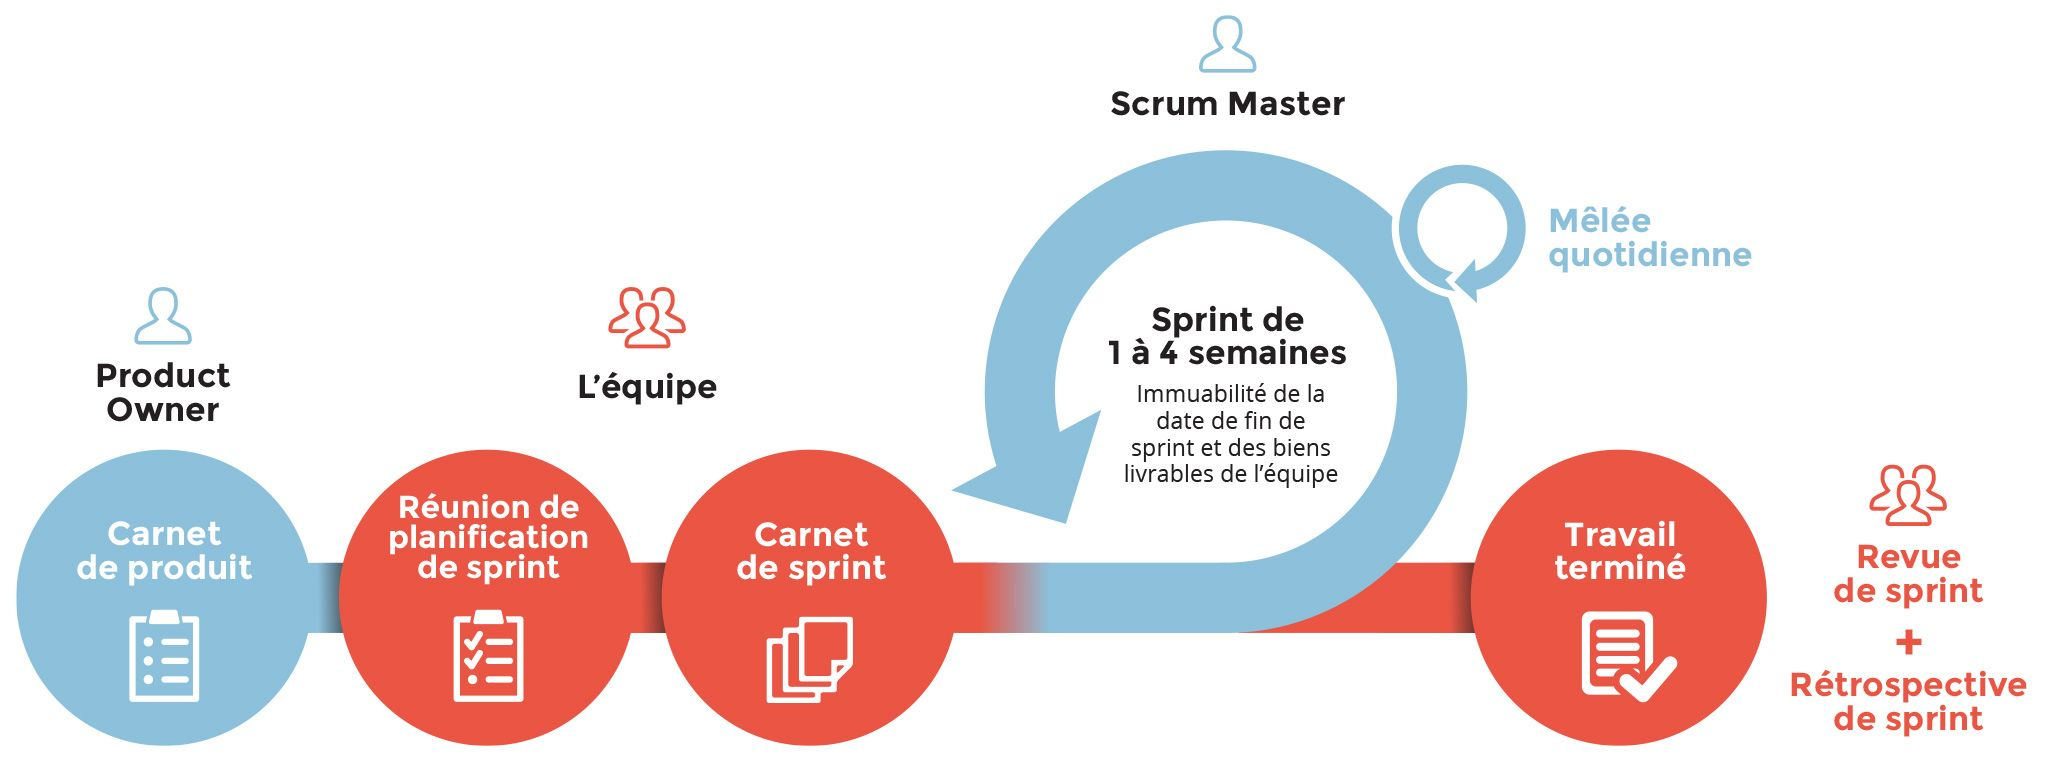
\includegraphics[scale=0.21]{images/scrum.jpeg}
\caption{Le cycle de vie en Scrum}
\label{scrumSpirale}
\end{figure}


\noindent \bfseries Les Rôles \mdseries : \\
Scrum définit trois rôles clés, indispensables à la réussite du projet :
\begin{itemize}
\item \noindent \bfseries Le Product Owner  \mdseries : Il est fréquent qu'un spécialiste de domaine assume le rôle de représentant officiel du client au sein d'un projet Scrum. Son rôle principal consiste à définir les besoins fonctionnels, établit les priorités dans le Product Backlog et veille à la satisfaction du client.\newline

\item \noindent \bfseries Le Scrum Master \mdseries : Garant de la méthode Scrum, il facilite le travail de l’équipe en supprimant les obstacles et en s’assurant que les pratiques agiles sont correctement appliquées.\\

\item \noindent \bfseries L’Équipe \mdseries : Les membres responsable de la conception, du développement, des tests et de la livraison des fonctionnalités à la fin de chaque sprint. Ils sont auto-organisés et multidisciplinaires. 
\end{itemize}

\noindent \bfseries Le Rythme Itératif \mdseries : 
\begin{itemize}
\item \noindent \bfseries Sprint  \mdseries : Le travail est organisé en cycles courts appelés sprints, d’une durée généralement comprise entre 2 et 4 semaines. À chaque sprint, une version incrémentale du produit est développée, testée et potentiellement livrable.

\end{itemize}

\noindent \bfseries Les Artefacts \mdseries : 
\begin{itemize}
\item \noindent \bfseries Product Backlog  \mdseries :  Liste hiérarchisée de toutes les fonctionnalités à développer, rédigées sous forme de User Stories. Ce backlog est régulièrement mis à jour en fonction des retours du client.

\item \noindent \bfseries Sprint Backlog  \mdseries : Sous-ensemble du Product Backlog sélectionné pour être réalisé lors d’un sprint donné. Il contient les User Stories détaillées et les tâches associées.
\end{itemize}
\newpage
\noindent \bfseries les Evénements \mdseries : 
\begin{itemize}
\item \noindent \bfseries Sprint Planning  \mdseries : Réunion de planification marquant le début de chaque sprint. L’équipe sélectionne les éléments à développer et définit les objectifs à atteindre.
\item \noindent \bfseries Daily Scrum (Mêlée quotidienne)  \mdseries : Courte réunion quotidienne, souvent appelée "stand-up" en raison de sa brièveté (15 minutes maximum), visant à synchroniser les efforts de l’équipe. Chaque membre partage trois points : ce qu’il a accompli depuis la dernière mêlée, ce qu’il prévoit de faire avant la prochaine, et les éventuels blocages rencontrés. Facilitée par le Scrum Master, cette rencontre n’est pas destinée à résoudre les problèmes sur-le-champ, mais à les identifier pour un traitement ultérieur. Elle favorise la transparence, renforce la collaboration et permet d’ajuster rapidement le plan du sprint si nécessaire.
\item \noindent \bfseries Definition of Done (DoD) \mdseries :
Ensemble de critères définissant qu’une tâche est considérée comme terminée (tests réussis, documentation rédigée, code relu, etc.).
\item \noindent \bfseries Definition of Ready (DoR) \mdseries :
Ce concept repose sur une compréhension commune des préparatifs requis pour une tâche, intégrant une liste de contrôle pour établir les User Stories. Pour être considérées comme prêtes à être mises en œuvre, les User Stories doivent répondre à plusieurs exigences, notamment la description exhaustive des scénarios d'utilisation, la disponibilité des ressources essentielles, des critères d'acceptation clairement définis et vérifiables, une taille adaptée, une présentation à l'équipe par le propriétaire du produit, des méthodes de test fonctionnelles, une estimation fiable de leur taille relative basée sur l'expérience utilisateur, ainsi que la spécification des appareils ciblés.

\item \noindent \bfseries Revue de Sprint  \mdseries : Réunion organisée à la fin de chaque sprint pour évaluer le travail accompli. L’équipe présente l’incrément terminé au Product Owner et aux parties prenantes, qui valident sa conformité aux attentes. Si nécessaire, des ajustements sont apportés au "Product Backlog" pour refléter l’évolution des besoins ou des priorités. D’une durée maximale de 4 heures pour un sprint d’un mois, cette étape vise à garantir que le projet progresse efficacement, tout en maintenant un alignement constant avec les objectifs stratégiques et les exigences changeantes.

\item \noindent \bfseries Rétrospective de Sprint  \mdseries : 
Rencontre tenue immédiatement après la revue, dédiée à l’amélioration continue. L’équipe, guidée par le Scrum Master, analyse le sprint écoulé en identifiant ce qui a bien fonctionné, les difficultés rencontrées, et les opportunités d’optimisation. Des actions concrètes sont définies pour le sprint suivant, comme ajuster les processus ou résoudre des blocages récurrents. Limitée à 3 heures pour un sprint d’un mois, cette réunion renforce l’auto-organisation de l’équipe et assure une progression constante dans la qualité et l’efficacité du travail.

\end{itemize}
\newpage
\section{Langage de modélisation : UML}
Le langage UML (Unified Modeling Language) est un langage standardisé de modélisation utilisé dans la conception orientée objet des systèmes logiciels. Il permet de représenter, visualiser, spécifier, construire et documenter de manière formelle les différents aspects d’un système, tant structurels que comportementaux.\\
\\
UML repose sur un ensemble de diagrammes graphiques permettant de décrire les éléments clés d’un système : les classes, les objets, les interactions, les activités, les cas d'utilisation, etc. Ces représentations facilitent la communication entre les différents acteurs du projet (développeurs, analystes, chefs de projet) et garantissent une compréhension commune du fonctionnement global du système.\\
\\
Dans le cadre de notre projet, nous avons choisi d’utiliser UML pour modéliser les différentes composantes de notre application. Ce choix s’explique par la richesse expressive d’UML, sa capacité à structurer efficacement un système complexe, et sa large adoption dans l’industrie comme outil de conception et de documentation. La figure \ref{umlLogo} présente le logo du language de modélisation UML.\\

\begin{figure}[H]
\centering
\includegraphics[scale=0.5]{images/UML_logo.png}
\caption{Interface de ClickUp}
\label{umlLogo}
\end{figure}
\section{Outils adoptés pour la gestion de projet}
\normalsize{
Pour assurer le succès de notre projet et garantir une livraison réussie de notre produit, nous avons mis en place un ensemble d'outils de gestion de projet stratégiques, parmi lesquels nous pouvons citer :
\begin{itemize}
    \item \noindent \bfseries Git \mdseries : Un système de contrôle de version permettant de suivre les modifications apportées aux fichiers de code, facilitant ainsi une collaboration fluide et efficace entre plusieurs contributeurs.
    \item \noindent \bfseries GitLab \mdseries : Une plateforme de gestion de dépôts basée sur Git, qui simplifie le suivi et l’organisation de nos ressources tout en optimisant leur gestion.
    \item \noindent \bfseries Microsoft Teams \mdseries : Un outil collaboratif de communication qui renforce les interactions au sein de l’équipe, favorisant une coordination transparente et une communication améliorée.
    \newpage
    \item \noindent \bfseries ClickUp \mdseries : Une solution open source de gestion de projet, essentielle pour planifier, suivre et gérer les tâches, contribuant ainsi à une administration efficace et structurée de l’ensemble du projet. La figure \ref{clickup} présente l'interface de ClickUp.
\end{itemize}

\begin{figure}[H]
\centering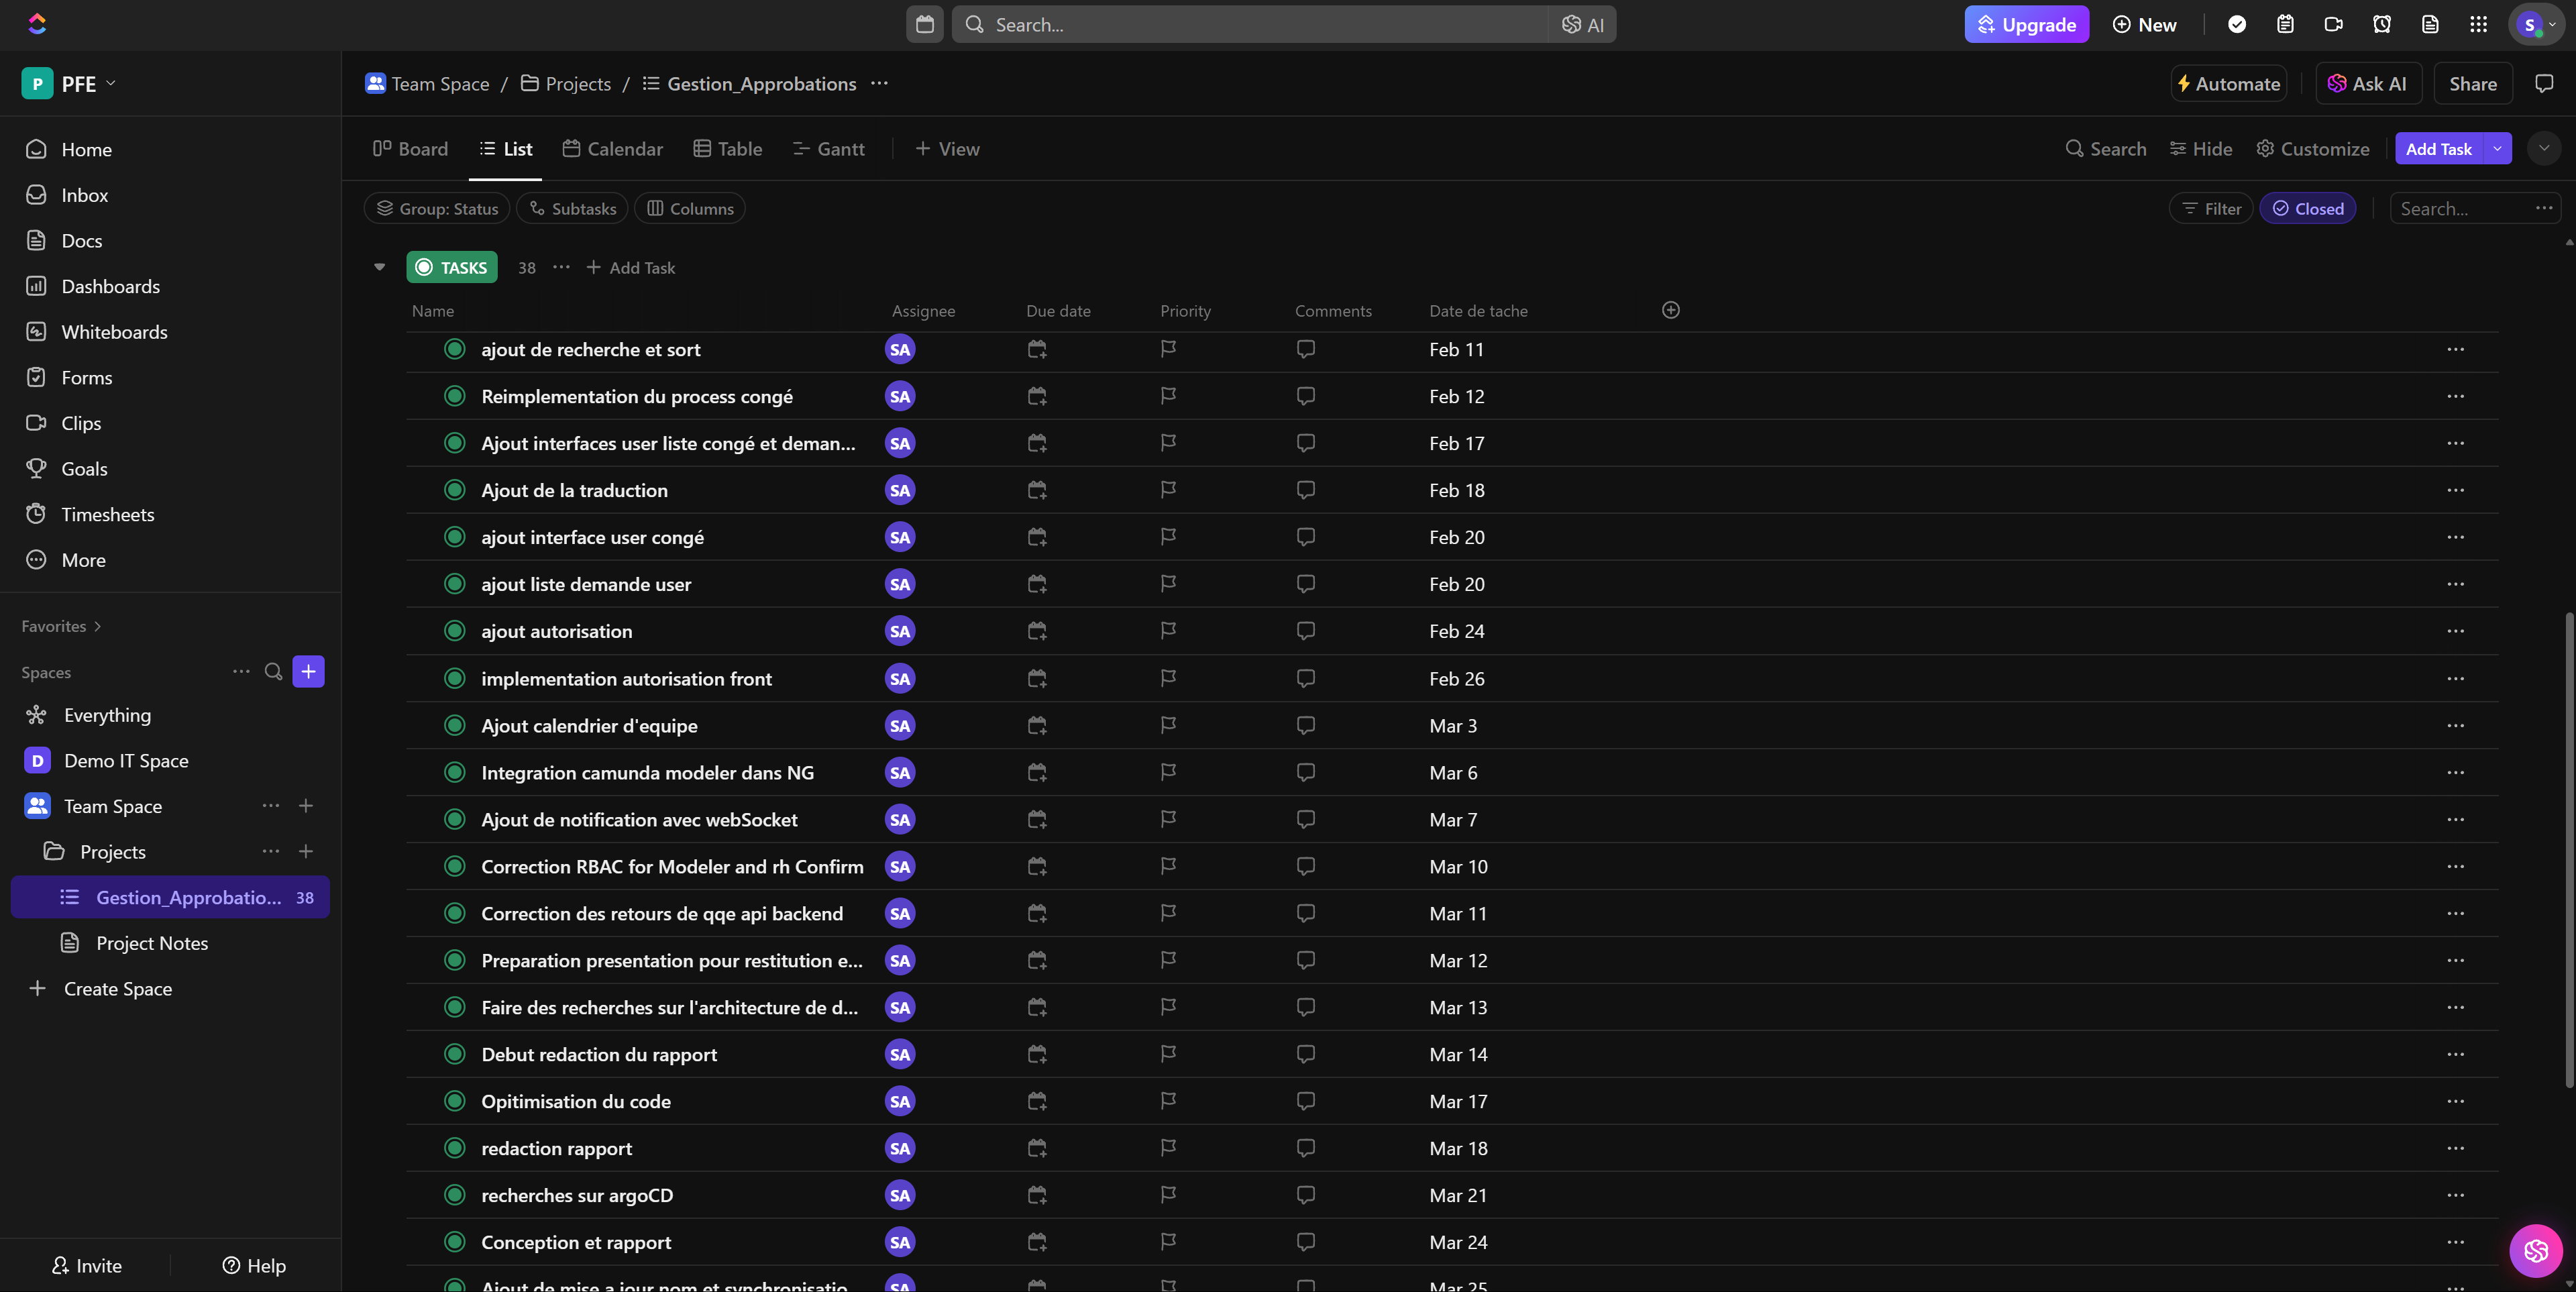
\includegraphics[scale=0.32]{images/clickUp.png}
\caption{Interface de ClickUp}
\label{clickup}
\end{figure}

\section*{Conclusion}

\normalsize{

Dans ce premier chapitre, nous avons introduit l’organisme d’accueil tout en offrant un aperçu général de la problématique et des objectifs du projet. \\
Nous avons également décrit la méthodologie retenue ainsi que le formalisme encadrant le processus mis en œuvre pour le développement de notre application. \\
Le chapitre suivant se concentrera sur l’analyse de la solution existante, en mettant en lumière ses limites et en proposant une nouvelle solution à concevoir.

}

}
}
